\documentclass[11pt]{article} % Type of document and font size
% \renewcommand{\baselinestretch}{1,15} % Specify line spacing
\usepackage[margin=2.5cm]{geometry} % Précise les marges du document
\usepackage[utf8]{inputenc}	% Précise comment le texte est saisi : cela permet de tapper directement les accents
\usepackage[english]{babel} % For English
% \usepackage[T1]{fontenc}	% Précise la façon dont le document actuel est encodé
\usepackage{setspace}
\usepackage{indentfirst} % To indent the first paragraph
% \usepackage{natbib} % To have bilbiography
\usepackage{csquotes}
\usepackage[sorting=none]{biblatex} % Bibliography
\addbibresource{ref.bib}
\usepackage[toc,page]{appendix} % Appendix


%Autres packages et commandes utiles
%----------------------------------------------------------------
\usepackage{enumerate} % Pour mieux gérer la commande enumerate dans les sections
\usepackage{graphicx}	% Pour inclure des images
\usepackage{float}
\graphicspath{ {./images/} } % set path to images
\usepackage{hyperref} % to allow hyperlinks
\usepackage{typed-checklist} % for checklist

%Titre
%----------------------------------------------------------------
\title{IFT-7030 Project proposal}
\author{Philippe Gélinas 536 782 326 \\ Antoine Reid 536 899 522}
\date{\vspace{-5ex}} % Don't show date and remove spacing

%----------------------------------------------------------------
\begin{document}

\maketitle

\section*{Abstract}
The project aims to compare different approaches to fine-tune a multimodal large language models (MLLM) for multimodal multiple-choice question answering on the ScienceQA dataset \cite{ScienceQA}. More recent fine-tuning approaches will be explored and compared to traditional fine-tuning. We will use accuracy to compare model performance.

\section*{Introduction}
We will compare different ways to fine-tune an MLMM for multimodal multiple-choice question answering. In this type of task, a multiple-choice question is asked which references a given image. We will use the ScienceQA dataset as a benchmark. This dataset contains primary and high-school questions related to science and is easily available on HuggingFace.

The first fine-tuning method will consist of a two-step fine-tuning method. Since the ScienceQA dataset contains a relatively small amount of data for NLP tasks (21k observations), we will first try to improve the reasoning abilities of the MLMM by performing supervised fine-tuning. We will use a larger dataset for this such as SearchQA (a collection of 140k Jepoardy! questions), HotpotQA (113k reasoning questions from Wikipedia articles), or Orca-Math (a dataset containing roughly 200k grade school math problems). After this first round of fine-tuning, the MLLM will then be fine-tuned to specialize in multiple-choice question answering with the ScienceQA dataset using regular fine-tuning. Regular fine-tuning consists of freezing all but the attention layer and updating weights.

Another fine-tuning approach we will explore is QLoRA \cite{qlora}. This deviates from traditional fine-tuning by representing the weight update matrix ($\Delta W$) as a low-rank decomposition of the weight matrix. This approach requires much less computational resources than traditional fine-tuning.

We will also explore fine-tuning using DoRA \cite{dora}, which is a LoRa \cite{lora} variant like QLoRA. Its authors claim that it is a better approach to fine-tuning than LoRa, while still maintaining the computational advantage of LoRA.

If we have time, we will compare with a training approach using retrieval-augmented generation (RAG). RAGs can help improve the capabilities of LLMs on specific domains by referencing knowledge outside of the training sources of the LLM.

\section*{Literature review} 
LoRA (Low-Rank Adaptation) is a fine-tuning technique for LLMs introduced by \cite{lora}. It deviates from regular fine-tuning by freezing the original model weights and by updating a separate set of weights which are then added to the original weights. In regular fine-tuning an entire weight update matrix ($\Delta W$) is combined with the pre-trained weights. LoRA separates $\Delta W$ into 2 low-rank matrices that approximate it. This method significantly reduces the number of trainable parameters. Along with the reduced computational load this brings, it can also help prevent overfitting. The downside of LoRA is that it introduces a new hyperparameter, $r$, which must be optimized. This hyperparameter represents the inner dimension of the low-rank matrices. QLoRA \cite{qlora} is a modification of LoRA that introduces increased memory efficiency due to storing weight parameters with 4-bit precision. \cite{qlora} observed performance levels similar to those of LoRA.
Another LoRa variant is DoRA \cite{dora}, which is supposed to outperform LoRa for fine-tuning LLMs for various tasks, including ours, which relates to image-text understanding. DoRA decomposes the weights of a pre-trained model into magnitude and direction components. For more details about DoRA, see appendix \ref{appendix:dora}.

An extensive review of RAG \cite{ragreview} has found that RAGs can help address hallucination and outdated knowledge problems. The advantage of RAG is that they allow for continuous knowledge update to the model and can allow an LLM to incorporate knowledge outside of the training domain. RAG are not always better than fine-tuning, especially for tasks which require specific data formats as inputs and a response in a particular style.

\section*{Input-Output Dataset}

As mentioned, we will use the ScienceQA dataset. The ScienceQA dataset contains 21\,208 multimodal multiple-choice questions collected from primary and high school curricula. The questions are separated into 3 subjects: natural science, language science, and social science. Roughly 49\,\% of the questions have an image context, 48\,\% have a text context, and 31\,\% have both. An interesting aspect of the ScienceQA dataset is that most question contain lectures (84\,\%) and detailed explanations (91\,\%) that help answer the question. The dataset has already been split into train, test, and validation sets on HuggingFace. The train set contains 12\,726 observations, whereas the test and validation sets each contains 4\,241 observations. We will use the train and tests sets to fine-tune the model and the test set to evaluate performance. The following diagram illustrates what the input (query) can look like and how it will be processed: 

\begin{figure}[H]
    \centering
    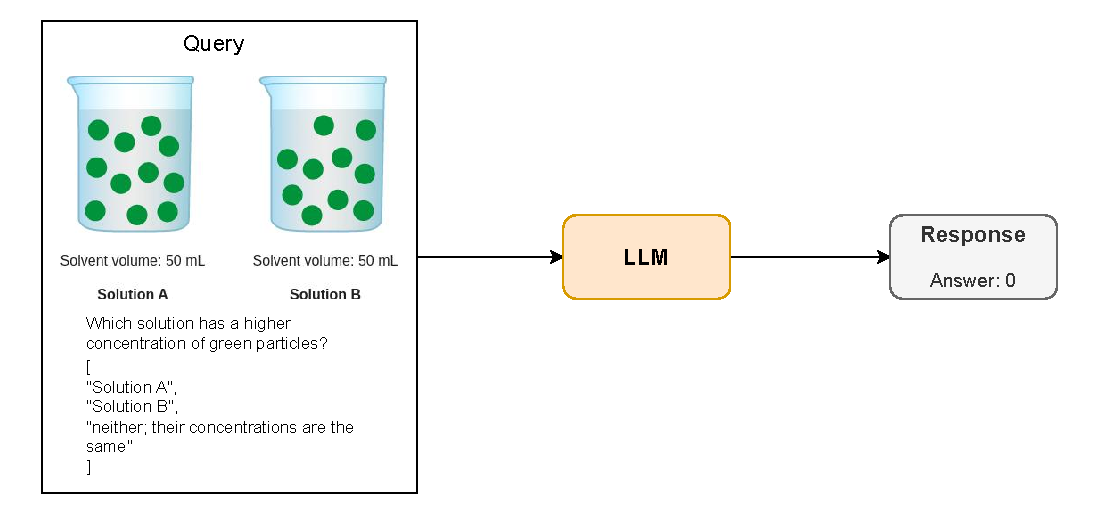
\includegraphics[width=\linewidth]{llm_diagram.pdf}
\end{figure}

There are 2 steps to this process :
\begin{enumerate}
    \item Pass the original query and the image to the LLM.
    \item Obtain response from the LLM. The response will be the index of the chosen answer from the list of choices (in the example the answer would be solution A).
\end{enumerate}

We will use a pretrained LLM as the base model. We must use a multimodal LLM as some queries can contain images. We will limit ourselves to LLMs with no more than 8 billion parameters to keep training times reasonable. Suitable MLLMs could be Qwen2VL \cite{Qwen2VL}, LLaVA \cite{liu2023llava}, or InternVL \cite{chen2023internvl}. 

\section*{Performance Metrics}
We will evaluate performance using accuracy. It is a widely used and suitable metric for multiple-choice question answering since it is simple and easily interpretable.

\section*{Computational Resources}
Fine-tuning an LLM requires good GPU resources to have reasonable training times. Given that the ScienceQA dataset is not extremely big and that we will limit ourselves to an LLM with no more than 8b parameters, the resources Valeria provides should be adequate. As a backup, our team has access to an NVIDIA RTX 4060 laptop GPU with 8 gigabytes of VRAM which should still manage to fine-tune a smaller sized LLM if trained overnight. 

\section*{Checklist}
\begin{CheckList}{Task}
    \Task{done}{Realistic} The dataset is being used is well defined and will require little pre-processing. The bulk of the time will be spent fine-tuning an LLM. With access to GPUs from Valeria and the ability to execute training for long periods, it is feasible to fine-tune an LLM multiple times.
    \Task{done}{Well defined dataset} The ScienceQA dataset is available on HuggingFace. Each question has an identified correct answer and, when applicable, an associated image and context.
    \Task{done}{Clearly define input and output} The input the LLM will receive is a multiple-choice question along with a list of possible answers. The output will be an index of the answer list that corresponds to the chosen answer.
    \Task{done}{Not be trivial} LLM fine-tuning is far from being a trivial task. LLMs are still not fully understood and research is still being done to optimize their fine-tuning. 
    \Task{done}{Within machine learning and/or signal processing domain} NLP tasks such as QA lie within the signal processing domain. Using a transformer model to solve the task also means that it lies within the machine learning domain.
    \Task{done}{Well situated within the literature} Many articles have been published on the topic of fine-tuning LLMs. It is still an active research subject and new fine-tuning methods are constantly being explored.
\end{CheckList}

% References
\medskip
\printbibliography

\newpage

% Appendix
\begin{appendices}
    \section{DoRA}\label{appendix:dora}
    The following figure taken from \cite{dora} explains in greater detail how weights are updated in the DoRA architecture.
    \begin{figure}[H]
        \centering
        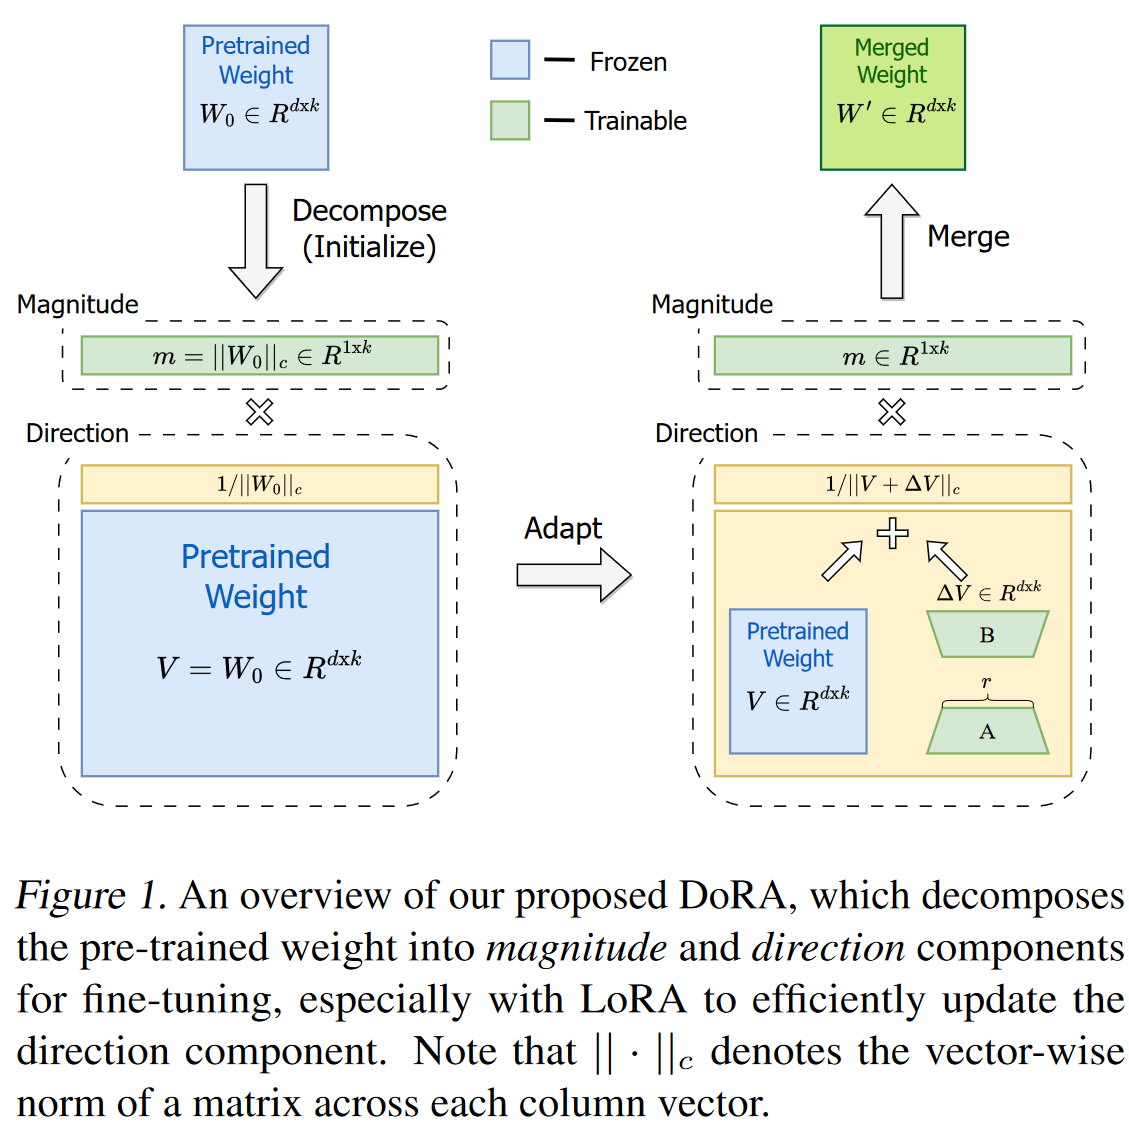
\includegraphics[scale=0.6]{dora_diagram.png}
    \end{figure}
    

\end{appendices}

\end{document}